\subsection{センサノードの参加・離脱時の振る舞い}
いくつかのセンサノードが,グループへ参加・離脱する際の手法を述べる.新規センサノードがグループに参加するため,GLノードはデータ集約時以外は,Adv Packetに自身のBLEサービスUUIDを載せAdvを行う.新規センサノードは,起動時にBLEスキャンを実行し周囲に参加可能なグループがあるか探索する.発見した場合は,そのグループに参加し,そうでない場合はLoRaWANで直接センサデータを送信する.ノードが故障や電池切れで離脱する場合は,NSがデバイスを管理しているので,N回通信が来なかった場合に,グループリストからセンサノードを取り除く.GLノードの次回通信時に,更新したグループリストを通知する.


\begin{figure}[]
    \begin{center}
    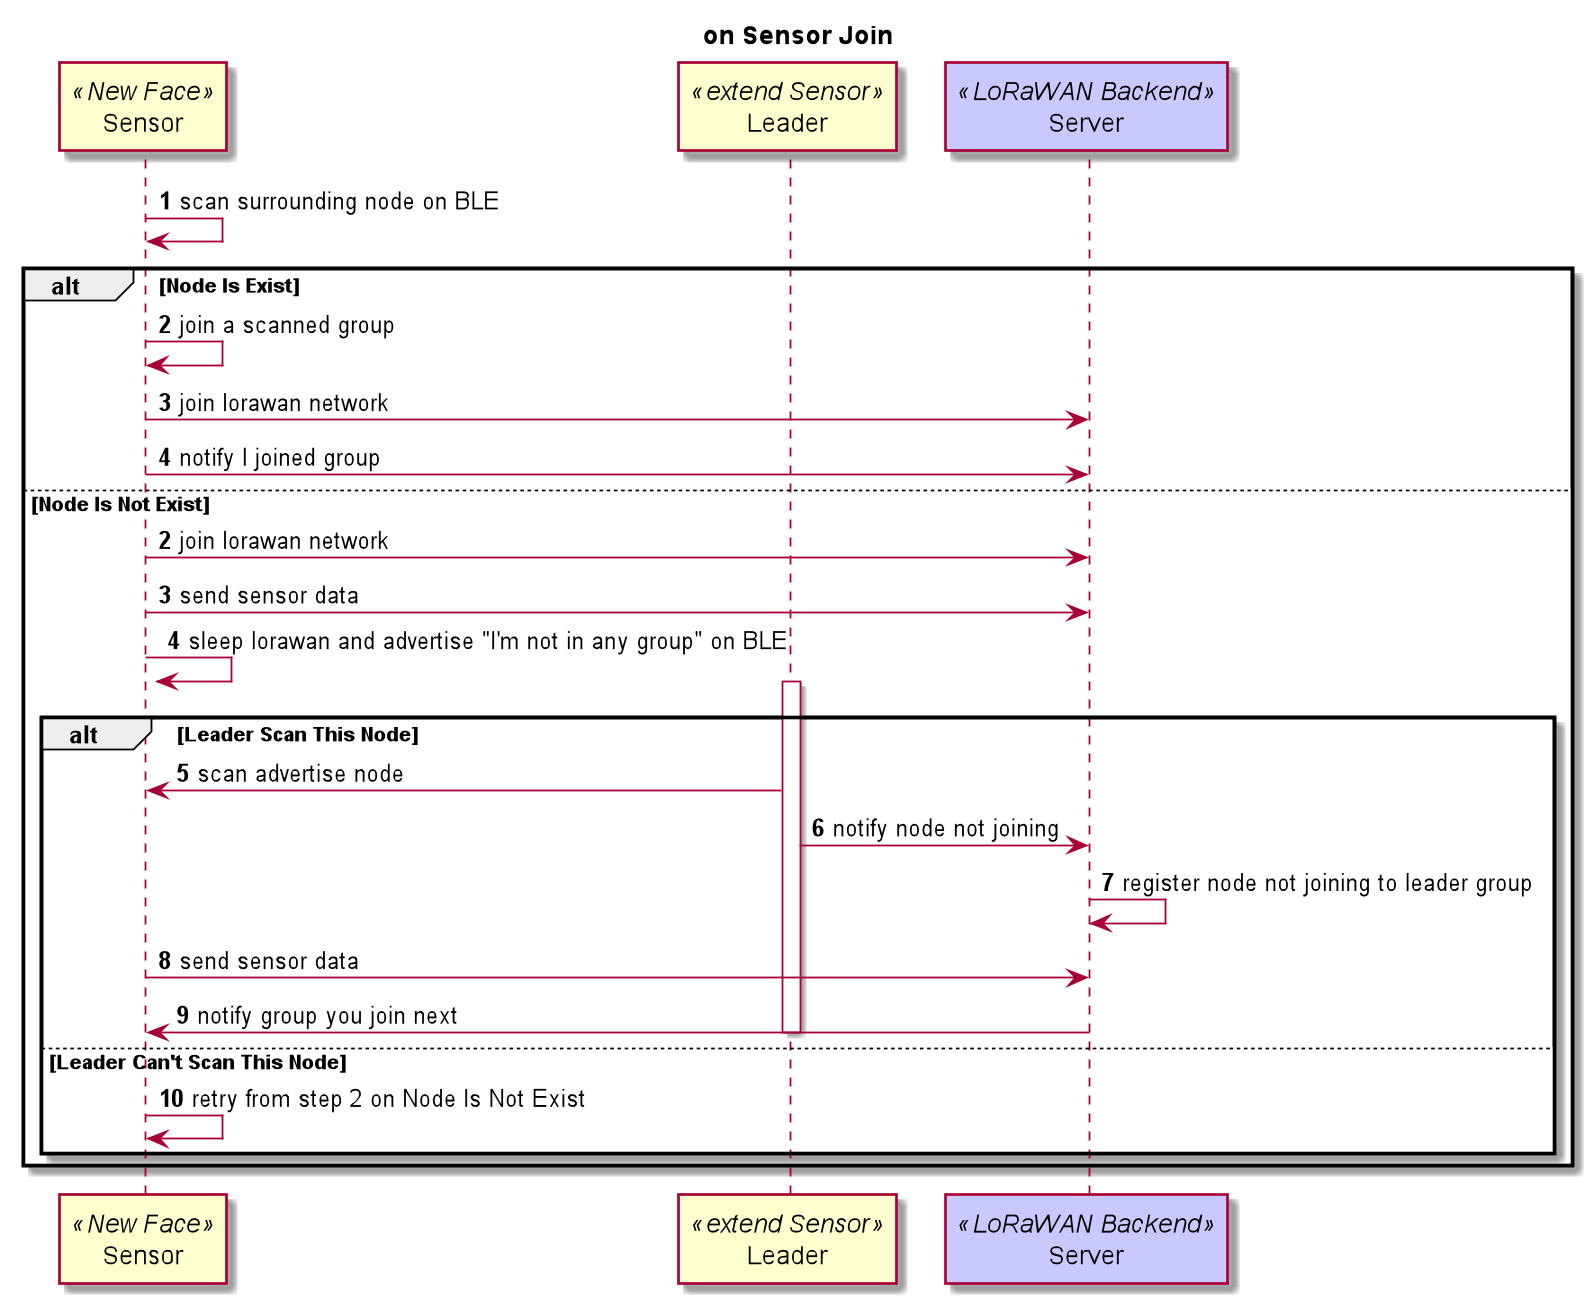
\includegraphics[width=14cm]{figures/グループ化_ネットワーク参加時.png}
    \caption{ネットワーク参加時の振る舞い}
    \label{fig:group_on_join}
    \end{center}
\end{figure}


\begin{figure}[]
    \begin{center}
    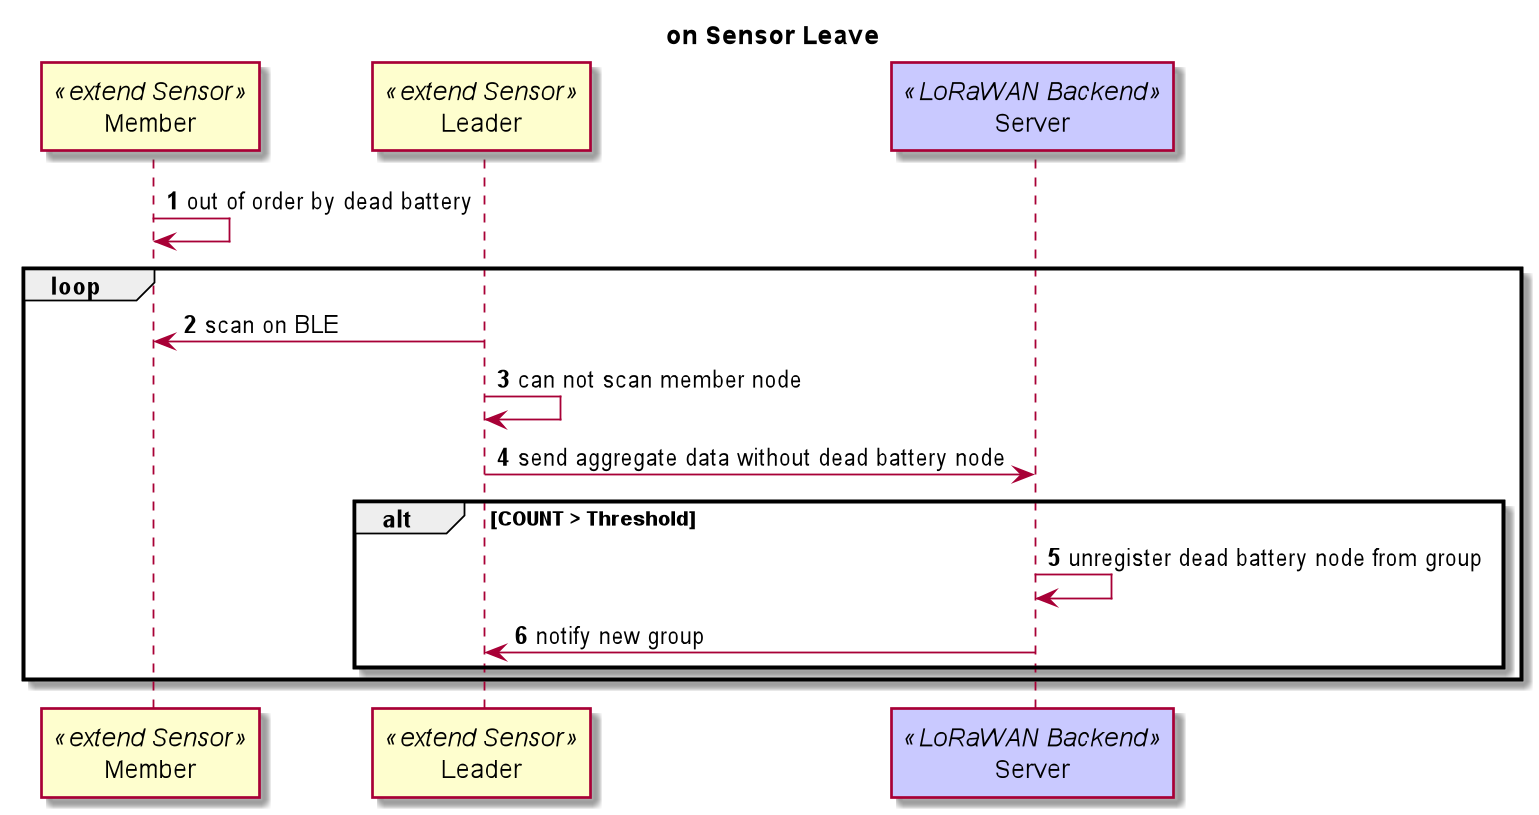
\includegraphics[width=14cm]{figures/グループ化_ネットワーク離脱時.png}
    \caption{ネットワーク離脱時の振る舞い}
    \label{fig:group_on_leave}
    \end{center}
\end{figure}